\documentclass[notes,11pt, aspectratio=169]{beamer}

\usepackage{pgfpages}
% These slides also contain speaker notes. You can print just the slides,
% just the notes, or both, depending on the setting below. Comment out the want
% you want.
\setbeameroption{hide notes} % Only slide
%\setbeameroption{show only notes} % Only notes
%\setbeameroption{show notes on second screen=right} % Both

\usepackage{helvet}
\usepackage[default]{lato}
\usepackage{array}
\usepackage{tgbonum}

\usepackage{tikz}
\usepackage{verbatim}
\setbeamertemplate{note page}{\pagecolor{yellow!5}\insertnote}
\usetikzlibrary{positioning}
\usetikzlibrary{snakes}
\usetikzlibrary{calc}
\usetikzlibrary{arrows}
\usetikzlibrary{decorations.markings}
\usetikzlibrary{shapes.misc}
\usetikzlibrary{matrix,shapes,arrows,fit,tikzmark}
\usepackage{amsmath}
\usepackage{mathpazo}
\usepackage{hyperref}
\usepackage{lipsum}
\usepackage{multimedia}
\usepackage{graphicx}
\usepackage{multirow}
\usepackage{graphicx}
\usepackage{dcolumn}
\usepackage{bbm}
\newcolumntype{d}[0]{D{.}{.}{5}}

\usepackage{changepage}
\usepackage{appendixnumberbeamer}
\newcommand{\beginbackup}{
   \newcounter{framenumbervorappendix}
   \setcounter{framenumbervorappendix}{\value{framenumber}}
   \setbeamertemplate{footline}
   {
     \leavevmode%
     \hline
     box{%
       \begin{beamercolorbox}[wd=\paperwidth,ht=2.25ex,dp=1ex,right]{footlinecolor}%
%         \insertframenumber  \hspace*{2ex} 
       \end{beamercolorbox}}%
     \vskip0pt%
   }
 }
\newcommand{\backupend}{
   \addtocounter{framenumbervorappendix}{-\value{framenumber}}
   \addtocounter{framenumber}{\value{framenumbervorappendix}} 
}


\usepackage{graphicx}
\usepackage[space]{grffile}
\usepackage{booktabs}
\newcommand\independent{\protect\mathpalette{\protect\independenT}{\perp}}
\def\independenT#1#2{\mathrel{\rlap{$#1#2$}\mkern2mu{#1#2}}}
\DeclareMathOperator{\Supp}{Supp}

% These are my colors -- there are many like them, but these ones are mine.
\definecolor{blue}{RGB}{0,114,178}
\definecolor{red}{RGB}{213,94,0}
\definecolor{yellow}{RGB}{240,228,66}
\definecolor{green}{RGB}{0,158,115}

\hypersetup{
  colorlinks=false,
  linkbordercolor = {white},
  linkcolor = {blue}
}


%% I use a beige off white for my background
\definecolor{MyBackground}{RGB}{255,253,218}

%% Uncomment this if you want to change the background color to something else
%\setbeamercolor{background canvas}{bg=MyBackground}

%% Change the bg color to adjust your transition slide background color!
\newenvironment{transitionframe}{
  \setbeamercolor{background canvas}{bg=yellow}
  \begin{frame}}{
    \end{frame}
}

\setbeamercolor{frametitle}{fg=blue}
\setbeamercolor{title}{fg=black}
\setbeamertemplate{footline}[frame number]
\setbeamertemplate{navigation symbols}{} 
\setbeamertemplate{itemize items}{-}
\setbeamercolor{itemize item}{fg=blue}
\setbeamercolor{itemize subitem}{fg=blue}
\setbeamercolor{enumerate item}{fg=blue}
\setbeamercolor{enumerate subitem}{fg=blue}
\setbeamercolor{button}{bg=MyBackground,fg=blue,}



% If you like road maps, rather than having clutter at the top, have a roadmap show up at the end of each section 
% (and after your introduction)
% Uncomment this is if you want the roadmap!
% \AtBeginSection[]
% {
%    \begin{frame}
%        \frametitle{Roadmap of Talk}
%        \tableofcontents[currentsection]
%    \end{frame}
% }
\setbeamercolor{section in toc}{fg=blue}
\setbeamercolor{subsection in toc}{fg=red}
\setbeamersize{text margin left=1em,text margin right=1em} 

\newenvironment{wideitemize}{\itemize\addtolength{\itemsep}{10pt}}{\enditemize}

\usepackage{environ}
\NewEnviron{videoframe}[1]{
  \begin{frame}
    \vspace{-8pt}
    \begin{columns}[onlytextwidth, T] % align columns
      \begin{column}{.70\textwidth}
        \begin{minipage}[t][\textheight][t]
          {\dimexpr\textwidth}
          \vspace{8pt}
          \hspace{4pt} {\Large \sc \textcolor{blue}{#1}}
          \vspace{8pt}
          
          \BODY
        \end{minipage}
      \end{column}%
      \hfill%
      \begin{column}{.38\textwidth}
        \colorbox{green!20}{\begin{minipage}[t][1.2\textheight][t]
            {\dimexpr\textwidth}
            Face goes here
          \end{minipage}}
      \end{column}%
    \end{columns}
  \end{frame}
}

\title[]{\textcolor{blue}{Potential Outcomes and Directed Acylic Graphs}}
\author[PGP]{}
\institute[FRBNY]{\small{Paul Goldsmith-Pinkham}}
\date{\today}


\begin{document}

%%% TIKZ STUFF
\tikzset{   
        every picture/.style={remember picture,baseline},
        every node/.style={anchor=base,align=center,outer sep=1.5pt},
        every path/.style={thick},
        }
\newcommand\marktopleft[1]{%
    \tikz[overlay,remember picture] 
        \node (marker-#1-a) at (-.3em,.3em) {};%
}
\newcommand\markbottomright[2]{%
    \tikz[overlay,remember picture] 
        \node (marker-#1-b) at (0em,0em) {};%
}
\tikzstyle{every picture}+=[remember picture] 
\tikzstyle{mybox} =[draw=black, very thick, rectangle, inner sep=10pt, inner ysep=20pt]
\tikzstyle{fancytitle} =[draw=black,fill=red, text=white]
%%%% END TIKZ STUFF

% Title Slide
\begin{frame}
\maketitle

\end{frame}

% INTRO
\begin{frame}{Causality and counterfactuals}
\begin{columns}[T] % align columns
\begin{column}{.58\textwidth}
  \begin{wideitemize}
  \item Not every economics research paper
    is estimating a causal quantity
    \begin{itemize}
    \item But, the implication or takeaway of papers is (almost) always
      a causal one
    \end{itemize}
  \item Causality lies at the heart of every exercise
  \item Goal for today's class:
    \begin{enumerate}
    \item Enumerate tools used to discuss causal questions
    \item Emphasize a \emph{multimodal} approach
    \item Set terminology/definitions for future discussions
    \end{enumerate}
  \end{wideitemize}
\end{column}%
\hfill%
\begin{column}{.38\textwidth}
  \vfill
  ``We do not have knowledge of a thing until we have grasped its why, that is to say, its cause.''\\
\hfill  -Aristotle

\end{column}%
\end{columns}
\end{frame}
%   \makebox[\linewidth][c]{
%     \resizebox{\linewidth}{!}{
% %      \includegraphics{how-to-draw-an-owl.pdf}
%     }}

% INTRO
\begin{frame}{Causality and counterfactuals - strong opinions}
\begin{columns}[T] % align columns
\begin{column}{.65\textwidth}
  \begin{wideitemize}
  \item The true underpinnings of causality are nearly philosphical in nature
    \begin{itemize}
    \item If Aristotle didn't settle the question, neither will
      researchers in the 21t century
    \end{itemize}
  \item I will avoid many of the discussions, but my biases will show up in one or two settings
  \item Key point: economics research is messy, and a careful
    discussion of causality entails two dimensions:
    \begin{enumerate}
    \item A good framework to articulate your assumptions
    \item Readers that understand the framework
    \end{enumerate}
  \end{wideitemize}
\end{column}%
\hfill%
\begin{column}{.38\textwidth}

\end{column}%
\end{columns}
\end{frame}

\begin{frame}{The problem of causal inference: a medical example}
\begin{columns}[T] % align columns
\begin{column}{.8\textwidth}
  \begin{wideitemize}
    \item  Two variables:
    \begin{itemize}
    \item $Y \in \{0, 1\}$: whether a person will get Covid-19
    \item $D \in \{0, 1\}$: whether a person gets a vaccine
    \end{itemize}
  \item Our question: does $D$ causally affect $Y$?
  \item \emph{Ignore the question of data for now} -- this is purely a
    question of what is knowable.
  \item ``The fundamental problem of causal inference'' (Holland 1986)
    is that for a given individual, we can only observe one world --
    either they get the vaccine, or they do not
  \end{wideitemize}
\end{column}%
\hfill%
\begin{column}{.38\textwidth}
\end{column}%
\end{columns}
\end{frame}

\begin{frame}{The problem of causal inference: a medical example}
\begin{columns}[T] % align columns
\begin{column}{.65\textwidth}
  \begin{wideitemize}
  \item What is knowable?
    \begin{itemize}
    \item We need notation
    \item Begin with the Neyman-Rubin Causal model
    \end{itemize}
  \item There is a population of $n$ individuals, indexed by $i$. 
  \item Let $Y_{i}(D_{i})$ denote the outcome given a particular vaccine
    treatment
    \begin{itemize}
    \item  $Y_{i}(1)$: they receive the vaccine
    \item $Y_{i}(0)$: they do not receive the vaccine
    \end{itemize}
  \item \textbf{Key Assumption}? \pause person $i$'s outcome is only
    affected by their own treatment. We will discuss relaxing this
    assumption later.
    \begin{itemize}
    \item  SUTVA - Stable Unit Treatment Variable Assignment
    \end{itemize}
  \end{wideitemize}
\end{column}%
\hfill%
\begin{column}{.38\textwidth}

  \vspace{20pt}
  
  $Y_{i} = D_{i}Y_{i}(1) + (1-D_{i})Y_{i}(0)$\\
  \vspace{20pt}
  \begin{tabular}{ccccc}
    \toprule
    i & $Y_{i}(1)$ &  $Y_{i}(0)$ & $D_{i}$ & $Y_{i}$ \\
    \midrule
    1 &     1      &     0      &   1   & 1 \\
    2 &     0      &     0      &   1   & 0 \\
    3 &     1      &     0      &   0   & 0 \\
     & &  \vdots & & \\
    $n$ &     0      &     1      &   0   & 1 \\    
  \end{tabular}
\end{column}%
\end{columns}
\end{frame}

\begin{frame}{Causal inference is a missing data problem}
\begin{columns}[T] % align columns
\begin{column}{.65\textwidth}
  \begin{wideitemize}
  \item In the potential outcomes framework, causal inference and missing data are tightly linked.
  \item Any causal answer uses assumptions to infer the ``missing'' counterfactual 
  \item Goal of this course will be to discuss many ways to solve
    these types of problems
  \item Before diving into the many potential estimands, consider what
    the goal is.
    \begin{itemize}
    \item A structural parameter? E.g. $\text{dInvestment}/\text{dTax Rate}$
    \item Existence of an treatment effect?
    \item A policy evaluation?
    \end{itemize}
  \end{wideitemize}
\end{column}%
\hfill%
\begin{column}{.38\textwidth}

  \vspace{20pt}
  
  \vspace{20pt}
  
\end{column}%
\end{columns}
\end{frame}

\begin{frame}{A brief aside: estimands, estimators and estimates}
\begin{columns}[T] % align columns
\begin{column}{.65\textwidth}
  \begin{wideitemize}
  \item \underline{Estimand}: the quantity to be estimated
  \item \underline{Estimate}: the approximation of the estimand using a finite data sample
  \item \underline{Estimator}: the method or formula for arriving at the estimate for an estimand
  \item My way of remembering: \url{https://twitter.com/paulgp/status/1275135175966494721?s=20}
  \end{wideitemize}
\end{column}%
\hfill%
\begin{column}{.38\textwidth}

  \vspace{20pt}
  
  \vspace{20pt}
  
\end{column}%
\end{columns}
\end{frame}



\begin{frame}{Causal estimands}
\begin{columns}[T] % align columns
\begin{column}{.85\textwidth}
  \begin{wideitemize}
  \item We will start with the \underline{Average Treatment Effect}:
    \begin{itemize}
    \item $\tau_{ATE} = \mathbb{E}(\tau_{i}) = \mathbb{E}(Y_{i}(1) - Y_{i}(0)) = \mathbb{E}(Y_{i}(1)) - \mathbb{E}(Y_{i}(0))$
    \end{itemize}
  \item This expression is defined over the full population, and
    includes individuals who may never recieve the treatment.
    \begin{itemize}
    \item \underline{Average Treatment Effect on the Treated} $\tau_{ATT} = \mathbb{E}(\tau_{i} | D_{i} = 1) = \mathbb{E}(Y_{i}(1) - Y_{i}(0) | D_{i} = 1) = \mathbb{E}(Y_{i}(1) | D_{i} = 1) - \mathbb{E}(Y_{i}(0) | D_{i} = 1)$
    \item Estimated effect for individuals who \emph{received} the treatment.
    \item Note that one piece of this measure is purely observed data: $\mathbb{E}(Y_{i}(1) | D_{i} = 1)$
    \end{itemize}
  \item \underline{Conditional Average Treatment Effect}:  $\tau_{CATE}(x) = \mathbb{E}(\tau_{i} | X_{i} = x) = \mathbb{E}(Y_{i}(1) - Y_{i}(0) |  X_{i} = x)$ where $X_{i}$ is some additional characteristic. 
  \end{wideitemize}
\end{column}%
\hfill%
\begin{column}{.38\textwidth}
\end{column}%
\end{columns}
\end{frame}

\begin{frame}{A second brief aside: what is identification?}
\begin{columns}[T] % align columns
\begin{column}{.6\textwidth}
  \begin{wideitemize}
  \item What does (point) identification mean?
    \pause
  \item Intuitively, for an estimate of interest,
    $\tau_{ATE}$, to be identified, it means that in a world
    with no uncertainty about data, can we always identify the value
    of $\tau$ from the data we observe?
    \begin{itemize}
    \item In other words, it's an invertability condition
    \end{itemize}
  \end{wideitemize}
\end{column}%
\hfill%
\begin{column}{.38\textwidth}
  \vspace{20pt}
``Econometric identification really means
just one thing: model parameters or
features being uniquely determined from
the observable population that generates
the data''\\
\hfill -Lewbel (2019)
\end{column}%
\end{columns}

\pause
\vspace{5pt}
\begin{itemize}
  \item Why would something not be identified if we only observe $(Y_{i}, D_{i})$?
    \begin{itemize}
    \item Consider $\tau_{ATT}$. $\mathbb{E}(Y_{i}(1)| D_{i}= 1)$ is
      identified, mechanically. What about $\mathbb{E}(Y_{i}(0) | D_{i} = 1)$?
    \item One approach: make an assumption on the relationship between $D_{i}$ and
      $(Y_{i}(1), Y_{i}(0))$.
    \end{itemize}
\end{itemize}
\end{frame}


\begin{frame}{Under what conditions is the ATE identified?}
\begin{columns}[T] % align columns
  \hspace{5pt} \begin{column}{.8\textwidth} \underline{\textbf{Strong
        Ignorability:}} $D_{i}$ is \emph{strongly ignorable} conditional on a vector  $\mathbf{X}_{i}$ if
    \begin{enumerate}
    \item $(Y_{i}(0), Y_{i}(1)) \independent D_{i} | \mathbf{X}_{i} $
    \item $\exists \epsilon > 0$ s.t. $\epsilon < \Pr(D_{i} = 1 | X_{i}) < 1-\epsilon_{i}$
    \end{enumerate}

    \begin{itemize}
    \item    The first condition asserts independence of the treatment from the ``potential'' outcomes
    \item The second condition asserts that there are both treated and untreated individuals
    \end{itemize}

    \begin{itemize}
    \item N.B. The term ``strong ignorability'' is much more precise than exogeneous
      \begin{itemize}
      \item But less commonly used in economics.
      \item You might instead say ``$D_{i}$ is conditionally randomly assigned.''
      \item If you \emph{might} even say $D_{i}$ is exogeneous.
      \end{itemize}
    \end{itemize}
      
\end{column}%
\hfill%
\begin{column}{.38\textwidth}
\end{column}%
\end{columns}
\end{frame}

\begin{frame}{When could we not identify the ATE?}
  \begin{columns}[T] % align columns
    \begin{column}{.65\textwidth}
      \begin{wideitemize}
      \item Intuitively, we understand why we typically can't estimate a  treatment effect
      \item Consider an unobservable variable, $U_{i} \in \{0, 1\}$ where $(Y_{i}(0) , Y_{i}(1), D_{i}) \not\independent U_{i}$
      \item Simple example: when
        $E(D_{i} | U_{i} = 1) > E(D_{i} | U_{i} = 0)$ and
        $E(\tau_{i} | U_{i} = 1) > E(\tau_{i} | U_{i} = 0)$.
      \item In other word, there is a variable that influences both
        the potential outcomes and the choice of treatment.
        \begin{itemize}
        \item In this case, estimating the counterfactual is
          contaminated by the variable $U_{i}$
        \end{itemize}
      \item Many of the goals in this class will be to address this
      \end{wideitemize}
\end{column}%
\hfill%
\begin{column}{.38\textwidth}
\end{column}%
\end{columns}
\end{frame}


\begin{frame}{Theorem: Identification of the ATE}
\begin{columns}[T] % align columns
  \hspace{5pt} \begin{column}{.8\textwidth}

    \underline{Theorem:} If $D_{i}$ is strongly ignorable conditional on $\mathbf{X}_{i}$, then
    $$\mathbb{E}(\tau_{i}) = \sum_{x \in \Supp X_{i}} (\mathbb{E}(Y_{i} | D_{i} = 1, \mathbf{X}_{i} = x) - \mathbb{E}(Y_{i} | D_{i} = 0, \mathbf{X}_{i} = x) )Pr(\mathbf{X}_{i} = x)$$
    \underline{Proof:} Note that
    $\mathbb{E}(Y_{i}(0) | \mathbf{X}_{i} ) = \mathbb{E}(Y_{i}(0) | D_{i} = 0, \mathbf{X}_{i} ) = \mathbb{E}(Y_{i}
    | D_{i} = 0, \mathbf{X}_{i})$ by strong ignorability. In essence,
    independence of $D_{i}$ and $(Y_{i}(0), Y_{i}(1))$ lets us
    interchange counterfactuals and realized data in conditionals. The
    rest follows by the law of iterated expectations. \qed

    \begin{itemize}
    \item Key implication -- counterfactual can be generated by using the averages. 
    \end{itemize}
  \end{column}%
  \hfill%
  \begin{column}{.38\textwidth}
  \end{column}%
\end{columns}
\end{frame}

\begin{frame}{Identification of the ATE - Intuition}
\begin{columns}[T] % align columns
  \begin{column}{.5\textwidth}
    \begin{center}
      \begin{tabular}{ccccc}
        \toprule
        $i$ & $Y_{i}(1)$ &  $Y_{i}(0)$ & $D_{i}$ & $Y_{i}$ \\
        \midrule
        1 &     1      &     -      &   1   & 1 \\
        2 &     0      &     -      &   1   & 0 \\
        3 &     1      &     -      &   1   & 1 \\
        4 &     1      &     -      &   1   & 1 \\
        5 &     -      &     0      &   0   & 0 \\
        6 &     -      &     0      &   0   & 0 \\
        7 &     -      &     0      &   0   & 0 \\        
        8 &     -      &     1      &   0   & 1 \\    
      \end{tabular}
    \end{center}
  \end{column}%
  \hfill%
  \begin{column}{.5\textwidth}
    \begin{wideitemize}
    \item We can estimate $\mathbb{E}(Y_{i} | D_{i} = 1) = 0.75$ and $\mathbb{E}(Y_{i} | D_{i} = 0) = 0.25$.
    \item We are defining our counterfactual in the missing data as 0.25, or 0.75, respectively.
    \item If we had covariates, we would condition within those groups.
    \item Note that this is all \emph{non-parametric} identification
      -- we have made no model restriction on the data-generating
      process
    \end{wideitemize}
  \end{column}
\end{columns}
\end{frame}

\begin{frame}{Identification through Directed Acylic Graphs (DAGs)}
\begin{columns}[T] % align columns
  \begin{column}{.5\textwidth}
    \begin{wideitemize}
    \item Above, we encoded random variables' relationships
      functionally, using potential outcomes
    \item An alternative approach does this graphically (with similar
      modeling under the hood -- to be continued...)
    \item We can encode the relationship between $D$ and $Y$ using an
      \emph{arrow} in a graph. The direction emphasizes that $D$
      causes $Y$, and not vice versa.
    \item Substantially more \emph{intuitive}
    \end{wideitemize}
  \end{column}%
  \hfill%
  \begin{column}{.5\textwidth}
    \begin{center}
      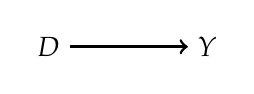
\begin{tikzpicture}
        \node[text centered] (t) {$D$};
        \node[right=1.5 of t, text centered] (y) {$Y$};
        \draw [->, line width= 1] (t) -- (y);
      \end{tikzpicture}
    \end{center}
  \end{column}
\end{columns}
\end{frame}

\begin{frame}{Identification through Directed Acylic Graphs (DAGs)}
\begin{columns}[T] % align columns
  \begin{column}{.5\textwidth}
    \begin{wideitemize}
    \item We can also allow for the unobservable $U$, which drove the identification concerns above
    \item In this case, $U$ is termed a \emph{confounder}. Why?
    \item Examine the paths by which $D$ links to $Y$:
      \begin{itemize}
      \item The standard direct effect $D \rightarrow Y$
      \item The ``Back-Door'' path $D \leftarrow U \rightarrow Y$
      \end{itemize}
    \item Note that the back-door is \emph{not} causal
    \item Key point: effect of $D$ on $Y$ is not identified under this setup
    \end{wideitemize}
  \end{column}%
  \hfill%
  \begin{column}{.5\textwidth}
    \begin{center}
      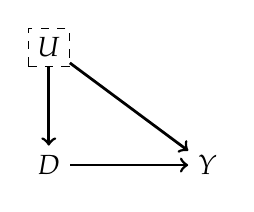
\begin{tikzpicture}
        % nodes %
        % \node[text centered] (z) {$Z$};
        \node[text centered] (t) {$D$};
        \node[right=1.5 of t, text centered] (y) {$Y$};
        \node[draw, rectangle, dashed, above = 1 of t, text centered] (u) {$U$};

        % edges %
        % \draw[->, line width= 1] (z) --  (t);
        \draw [->, line width= 1] (t) -- (y);
        % \draw[->,red, line width= 1,dashed] (u) --node {X} (z);
        \draw[->,line width= 1] (u) --(t);
        \draw[->,line width= 1] (u) -- (y);
%\draw[->, red, line width=1,dashed] (z) to  [out=270,in=270, looseness=0.5] node{X} (y);
      \end{tikzpicture}
    \end{center}
  \end{column}
\end{columns}
\end{frame}

\begin{frame}{Identification through Directed Acylic Graphs (DAGs)}
\begin{columns}[T] % align columns
  \begin{column}{.6\textwidth}
    \begin{wideitemize}
    \item We replace $U$ with an observable $X$
      identification concerns above
    \item $X$ is still a confounder, but we could condition on it and
      identify our effect. Why?
    \item Examine the paths by which $D$ links to $Y$:
      \begin{itemize}
      \item The standard direct effect $D \rightarrow Y$
      \item The ``Back-Door'' path $D \leftarrow X \rightarrow Y$
      \end{itemize}
    \item Now, conditioning on a variable along the path
      ``blocks'' the path
      \begin{itemize}
      \item E.g. $D$ is independent of $Y$ \emph{conditional} on $X$ (strong ignorability)
      \end{itemize}
    \end{wideitemize}
  \end{column}%
  \hfill%
  \begin{column}{.5\textwidth}
    \begin{center}
      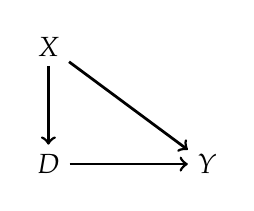
\begin{tikzpicture}
        % nodes %
        % \node[text centered] (z) {$Z$};
        \node[text centered] (t) {$D$};
        \node[right=1.5 of t, text centered] (y) {$Y$};
        \node[above = 1 of t, text centered] (u) {$X$};

        % edges %
        % \draw[->, line width= 1] (z) --  (t);
        \draw [->, line width= 1] (t) -- (y);
        % \draw[->,red, line width= 1,dashed] (u) --node {X} (z);
        \draw[->,line width= 1] (u) --(t);
        \draw[->,line width= 1] (u) -- (y);
%\draw[->, red, line width=1,dashed] (z) to  [out=270,in=270, looseness=0.5] node{X} (y);
      \end{tikzpicture}
    \end{center}
  \end{column}
\end{columns}
\end{frame}

\begin{frame}{Identification through Directed Acylic Graphs (DAGs)}
\begin{columns}[T] % align columns
  \begin{column}{.6\textwidth}
    \begin{wideitemize}
    \item One more example before formalizing the goal
      \begin{itemize}
      \item $X$ is now a ``collider'' (note direction of arrows)
      \end{itemize}
    \item Examine the paths by which $D$ links to $Y$:
      \begin{itemize}
      \item The standard direct effect $D \rightarrow Y$
      \item The path $D \rightarrow X \leftarrow Y$
      \end{itemize}
    \item Key difference: a collider is automatically blocked
      (if it or upstream variables are not conditioned on)
      \begin{itemize}
      \item If you condition on $X$, you open the path!
      \item Example: conditioning on an outcome variable
      \end{itemize}
    \end{wideitemize}
  \end{column}%
  \hfill%
  \begin{column}{.5\textwidth}
    \begin{center}
      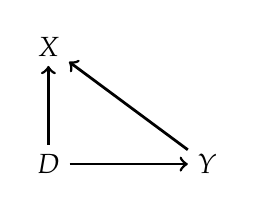
\begin{tikzpicture}
        % nodes %
        % \node[text centered] (z) {$Z$};
        \node[text centered] (t) {$D$};
        \node[right=1.5 of t, text centered] (y) {$Y$};
        \node[above = 1 of t, text centered] (u) {$X$};

        % edges %
        % \draw[->, line width= 1] (z) --  (t);
        \draw [->, line width= 1] (t) -- (y);
        % \draw[->,red, line width= 1,dashed] (u) --node {X} (z);
        \draw[<-,line width= 1] (u) --(t);
        \draw[<-,line width= 1] (u) -- (y);
%\draw[->, red, line width=1,dashed] (z) to  [out=270,in=270, looseness=0.5] node{X} (y);
      \end{tikzpicture}
    \end{center}
  \end{column}
\end{columns}
\end{frame}

\begin{frame}{Identification through Directed Acylic Graphs (DAGs)}
\begin{columns}[T] % align columns
  \begin{column}{.6\textwidth}
    \begin{wideitemize}
    \item<1-> The graphs looked similar, but the order of true causal path
      mattered
    \item<2-> Identifying colliders is a crucial aspect of identifying
      whether an effect is identified
    \item<3-> Key value in a DAG (to me) is laying out a model of
      causality, and clarifying what effects need to be restricted, even in a complicated setting
      \begin{itemize}
      \item For example, how is the effect of $D$ on $Y$ identified here?
      \end{itemize}
    \item<4-> What about now?
    \end{wideitemize}
  \end{column}%
  \hfill%
  \begin{column}{.5\textwidth}
    \begin{center}
\only<1>{      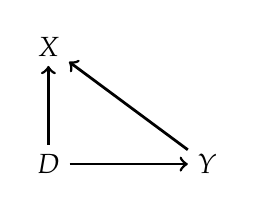
\begin{tikzpicture}
        % nodes %
        % \node[text centered] (z) {$Z$};
        \node[text centered] (t) {$D$};
        \node[right=1.5 of t, text centered] (y) {$Y$};
        \node[above = 1 of t, text centered] (u) {$X$};

        % edges %
        % \draw[->, line width= 1] (z) --  (t);
        \draw [->, line width= 1] (t) -- (y);
        % \draw[->,red, line width= 1,dashed] (u) --node {X} (z);
        \draw[<-,line width= 1] (u) --(t);
        \draw[<-,line width= 1] (u) -- (y);
%\draw[->, red, line width=1,dashed] (z) to  [out=270,in=270, looseness=0.5] node{X} (y);
      \end{tikzpicture}}
\only<2>{      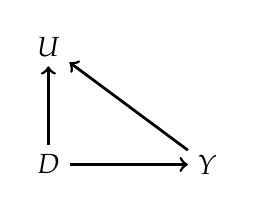
\begin{tikzpicture}
        % nodes %
        % \node[text centered] (z) {$Z$};
        \node[text centered] (t) {$D$};
        \node[right=1.5 of t, text centered] (y) {$Y$};
        \node[above = 1 of t, text centered] (u) {$U$};

        % edges %
        % \draw[->, line width= 1] (z) --  (t);
        \draw [->, line width= 1] (t) -- (y);
        % \draw[->,red, line width= 1,dashed] (u) --node {X} (z);
        \draw[<-,line width= 1] (u) --(t);
        \draw[<-,line width= 1] (u) -- (y);
%\draw[->, red, line width=1,dashed] (z) to  [out=270,in=270, looseness=0.5] node{X} (y);
      \end{tikzpicture}}
\only<3>{      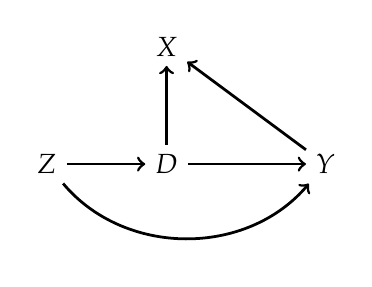
\begin{tikzpicture}
        % nodes %
        % \node[text centered] (z) {$Z$};
        \node[text centered] (t) {$D$};
        \node[right=1.5 of t, text centered] (y) {$Y$};
        \node[above = 1 of t, text centered] (u) {$X$};
        \node[left = 1 of t, text centered] (z) {$Z$};        
        % edges %
        % \draw[->, line width= 1] (z) --  (t);
        \draw [->, line width= 1] (t) -- (y);
        % \draw[->,red, line width= 1,dashed] (u) --node {X} (z);
        \draw[<-,line width= 1] (u) --(t);
        \draw[->,line width= 1] (z) --(t);
        \draw[->,bend right, line width= 1] (z) to [out=-50,in=-130]  (y);                
        \draw[<-,line width= 1] (u) -- (y);
%\draw[->, red, line width=1,dashed] (z) to  [out=270,in=270, looseness=0.5] node{X} (y);
      \end{tikzpicture}}
\only<4>{      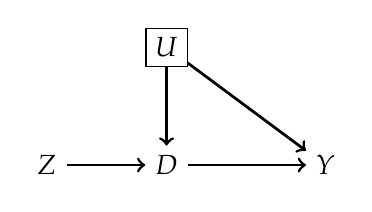
\begin{tikzpicture}
        % nodes %
        % \node[text centered] (z) {$Z$};
        \node[text centered] (t) {$D$};
        \node[right=1.5 of t, text centered] (y) {$Y$};
        \node[draw, above = 1 of t, text centered] (u) {$U$};
        \node[left = 1 of t, text centered] (z) {$Z$};        
        % edges %
        % \draw[->, line width= 1] (z) --  (t);
        \draw [->, line width= 1] (t) -- (y);
        % \draw[->,red, line width= 1,dashed] (u) --node {X} (z);
        \draw[->,line width= 1] (u) --(t);
        \draw[->,line width= 1] (z) --(t);
        \draw[->,line width= 1] (u) -- (y);
%\draw[->, red, line width=1,dashed] (z) to  [out=270,in=270, looseness=0.5] node{X} (y);
      \end{tikzpicture}}
    \end{center}
  \end{column}
\end{columns}
\end{frame}

\begin{frame}{Key steps with a DAG}
\begin{columns}[T] % align columns
  \begin{column}{.7\textwidth}
    \begin{wideitemize}
    \item Steps when using a DAG
      \begin{enumerate}
      \item Write down the DAG, and identify what effect you want
      \item Write all paths between the two nodes
      \item What are the ``causal'' paths (e.g. the arrows all flow in the right direction)?
      \item How many backdoor paths are there? Are they blocked? Can they be?
      \end{enumerate}
    \item Crucial point: conditioning on colliders will cause more harm than good
    \item We will revisit this setup for some empirical settings
      \begin{itemize}
      \item Let me know if you think there are good use cases!
      \end{itemize}
    \end{wideitemize}
  \end{column}%
  \hfill%
  \begin{column}{.5\textwidth}
  \end{column}
\end{columns}
\end{frame}

\begin{frame}{Structural equations and causal effects (Haile 2020)}
\begin{columns}[T] % align columns
  \begin{column}{.7\textwidth}
    \begin{wideitemize}
    \item \textbf{Important}: do not lose sight of the fact that these
      should be estimates that inform our economic model
    \item (Haile 2020) The reduced form equation is one where the
      inputs are i) \emph{exogeneous} (ed note: we have not defined
      this) and ii) unobservable (``structural errors'') and the outputs
      are endogeneous variables. [E.g. $Y_{i} = f(D_{i}, X_{i}, \epsilon_{i})$]
    \item The PO framework's key insight was considering the sets of
      counterfactuals for each individual. However, it is not magic;
      insights can typically map across different notations (DAGs, PO,
      structural econometric equations).  Note that these are
      effectively equivalent:
      \begin{align*}
        Y_{i} &= D_{i}Y_{i}(1) + (1-D_{i})Y_{i}(0)\\
        Y_{i} &= \alpha + D_{i}(\tau + v_{i}) + u_{i}        
      \end{align*}
    \end{wideitemize}
  \end{column}%
  \hfill%
  \begin{column}{.5\textwidth}
  \end{column}
\end{columns}
\end{frame}


\begin{frame}{Concrete example: demand and supply}
  \begin{wideitemize}
  \item Consider a demand and supply model: $P(Q)$ and $Q(P)$:
    \begin{align}
      P &= \alpha_{0} + \alpha_{1}Q + \alpha_{2}W + \epsilon\\
      Q &= \beta_{0} + \beta_{1}P + \beta_{2}V + \xi          
    \end{align}
  \item This is the ``structural'' equations
  \item The reduced form comes from plugging in the endogeneous
    variables and solving for only ``exogeneous'' variables on the RHS
  \item This will let us consider counterfactuals in the structural equations!
  \end{wideitemize}
  
\end{frame}

\end{document}